\documentclass{article}
\textheight = 21cm
\textwidth = 18cm
\topmargin = -2cm
\oddsidemargin= -2cm
\usepackage[T1]{fontenc}
\usepackage[utf8]{inputenc}
\usepackage{graphicx}
\usepackage[spanish]{babel}
\title{Tarea 1 Introducciòn a \Latex }
\date {\today }
\author{Diego Mèndez Medina }
\begin{document}   
\begin{center}
  
 
   {\fontsize{23}{0}\selectfont Introducción a las Ciencias de la Computación.}
  \\
  {\fontsize{23}{0}\selectfont Facultad de Ciencias, UNAM. }
  \\
  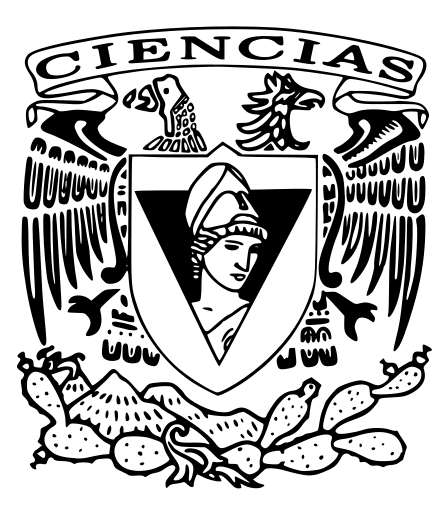
\includegraphics[width=3cm]{ciencias.png}\\
  \\
 {\fontsize{21}{0}\selectfont \fbox { Tarea 1: Introducción a \LaTeX . }} 
 \\
 {\fontsize{20}{0}\selectfont 
  Méndez Medina Diego, Grupo 702.  \\    }
Profesor : 	Salvador López Mendoza. \\	
Ayudante :	Marisol Amezcua. \\
Ayud. Lab. : 	Alejandro Iabin Arteaga Hernández.	
\end{center}
\begin{itemize}
\item {\bf Introducción Personal:} \\
Mi nombre es Diego Méndez Medina, tengo 19 años. Nací el 31 de Marzo del 2000. Cursé mi bachillerato en Voca 3, donde estudié la carrera de técnico en computación, la cual terminé en cuatro años. Me gusta mucho leer, mis libros favoritos son las autobiografías de Richard P. Feynman. Aunque también me gustan muchos los libros de Walter Isaacson, mi favorito suyo es ``los Inovadores'' en el cual cuenta la historia de la computación. Otro de mis pasatiempos es el deporte, en especial el soccer. Aunque ha pasado mucho tiempo sin que lo juegue lo he seguido y he sido fanático de los Pumas desde que tengo memoria. Ya como alumno de la UNAM espero aplicar mi descuento estudiantil e ir al mayor número de partidos que pueda y de ser posible entrar al equipo de la facultad. \\

\item {\bf Razones por las que elegí Ciencias de la Computación :} \\
  \begin{enumerate}
\item Al estudiar la carrera tecnica en computación me di cuenta que apesar de haber aprendido muchas cosas no me enseñaron lo que siempre me interesó, que son los fundamentos de la computación y verla más como una ciencia que como una ingieniería.

\item Mi plan era continuar mi educación en el IPN e ingresar a la carrera de matemáticas y física en la Escuela Superior de Físicas y Matemáticas(ESFM) para después buscar una maestría en computación, pero veía como un reto lograr pasar el examen de la UNAM.

\item Decidí estudiar Ciencias de la Computación por mi familia. Mi padre y madre estudiaron derecho en la UNAM, siempre le he ido a los pumas y mi novia, el amor de mi vida, que conozco desde la secundaria estudia historia en la Facultad de Filosofía y Letras. \\

\end{enumerate}
\item {\bf Optativas :}\\
\begin{itemize}
\item Computación Cuántica I y II. \\
\item Álgebra líneal II. \\
\item Análisis Combinatorio.\\
\item Cómputo de alto rendimiento.\\
\item Estadística I y II.\\
\item Geometría Computacional.\\
\item Lógica Computacional II.\\
\item Lenguajes de Programación II.\\
\item Lógica Matemática Iy II.\\
\item Introducción a las funciones recursivas y computabilidad.
\end{itemize}

\end{itemize}	
\end{document}
